\subsection{Procedure and prediction diagnostics}\label{app:internal-sage-F-details}
This study examines whether a shared bank produces better combined predictions than capable single models and complete ensembles. It extends factor placement into the native SAGE stack and evaluates the resulting training procedures on encountered WikiCS development. It is separate from the original five-dataset benchmark and the Roman component study.

The internal version places input and output factor vectors around every native dense map, including the input/output projectors, SAGE projections and feed-forward maps. Shared matrices and native biases remain trainable and retain their original initialization; private factor vectors distinguish four routes. The first input factors start with independent signs, and later factors start at one. Each route receives its own persistent dropout stream and makes a complete native graph pass. Unlike the original boundary projectors in Section~\ref{sec:method}, this version retains the shared native bias and also changes the internal maps. Factor placement, initialization and bias are therefore distinct parts of the recipe.

The fixed configuration uses two residual SAGE blocks, hidden width 128, LayerNorm, dropout 0.2 and AdamW with learning rate 0.001 and zero decay. Training minimizes mean ordinary member cross-entropy, with no pooled-loss gradient or context auxiliary. Prediction averages member class probabilities. Checkpoints maximize pooled development accuracy, retaining the earliest strict maximum, with a 1,000-update ceiling and 300-update stale patience.

The matched joint untied bank gives each route a complete private body. Its initial route functions, factor/dropout starts, mean-member objective and coherent pooled checkpoint selection match the shared bank. The genuine factorized independent ensemble has four complete bodies with separate native starts, optimizers, unscaled own losses and own checkpoint selectors, followed by probability averaging. Ordinary and factorized singles retain their own full losses and selectors. These five arms compare complete acquisition procedures; their parameter ownership and optimization histories differ.

All results below are means over three paired optimizer seeds on the same 5,274 development nodes used for checkpoint selection. Fixed five-fold temperature calibration follows native selection. These selected development readouts do not provide unused whole-pipeline confirmation.

\begin{figure}[t]
\centering
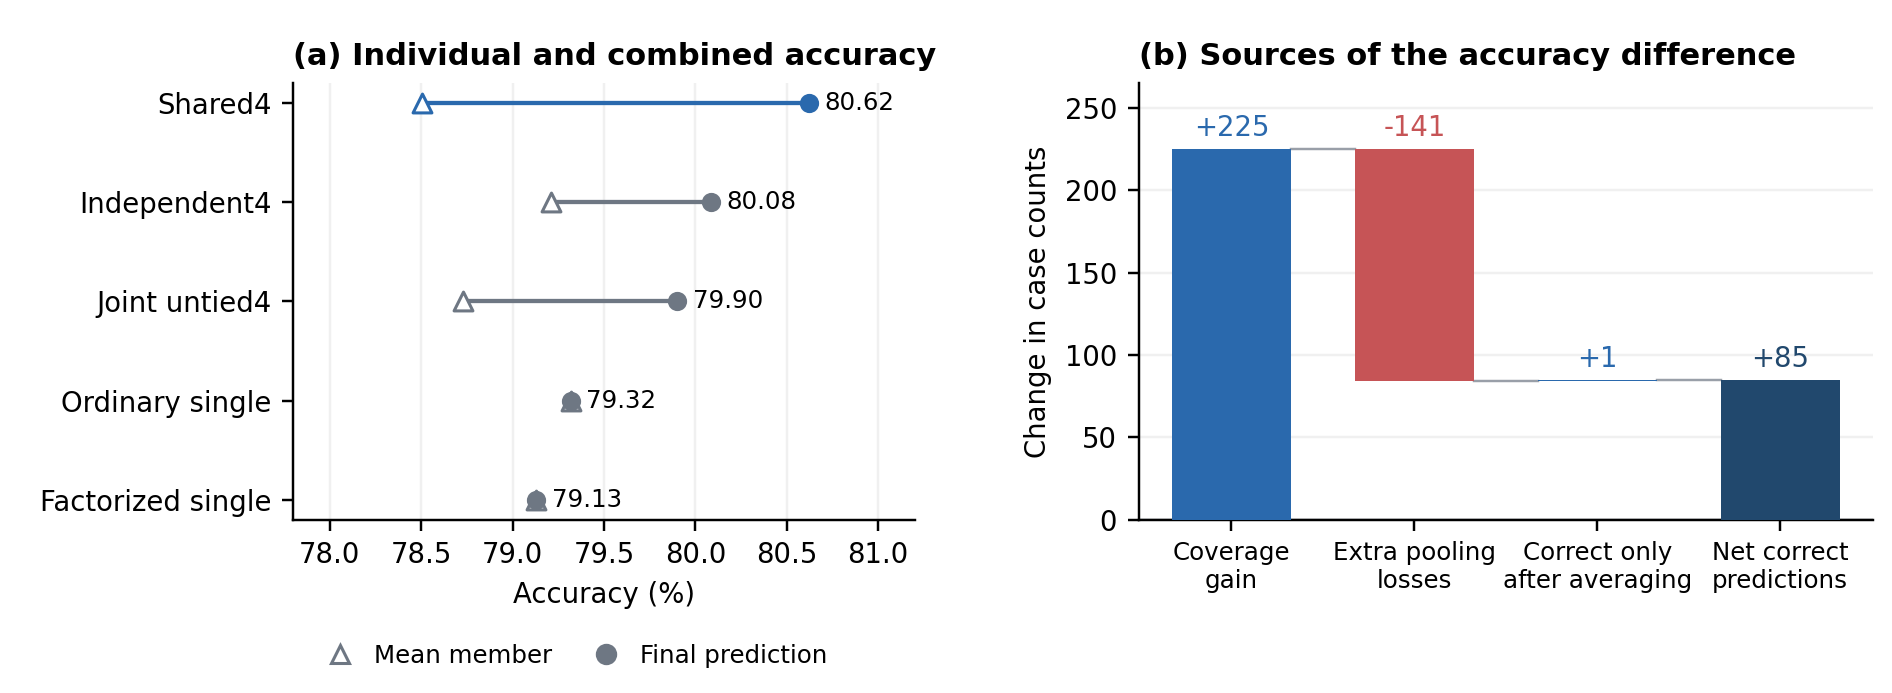
\includegraphics[width=\linewidth]{F_member_coverage_v2.png}
\caption{Internal SAGE on selected WikiCS development. (a) Shared4's average member is weaker than either complete ensemble control, while its combined prediction is more accurate. Both single-model references are shown. (b) Against independently acquired factorized models, 225 added covered cases are offset by 141 extra losses during averaging; one aggregation-only correction leaves 85 more correct decisions. Counts repeat the same 5,274 nodes across three optimizer seeds. The paired mean accuracy gain is 0.537 points, with a descriptive 95\% interval of $[-0.265,1.340]$; this is not unused confirmation or a statistically established superiority claim. Calibrated NLL is higher than that of the independent ensemble.}
\label{fig:internal-members-coverage}
\end{figure}

Shared4 has higher calibrated NLL than both ensemble controls, while calibrated Brier favors Shared4 over both. The accuracy benefit therefore accompanies a probability-quality tradeoff that differs across proper scores. Appendix~\ref{app:internal-sage-F} gives the absolute confidence metrics and the study's predeclared decision rules.

The main text reports the member/coverage comparison. Complete signed counts, gross repairs/harms and their original discussion remain in \path{code_evidence/native_F/complete_prediction_accounting.tex.txt}. These repeated-node diagnostics compare separately fitted and selected procedures and identify no general learning cause.

Fewer stored weights remain a secondary benefit: Shared4 has 216,674 parameters, versus 832,256 for the complete four-body controls. Its recorded acquisition sum is 71.676 seconds, versus 50.025 for joint untied4 and 58.620 for I4. These scopes include different stopping histories and do not establish lower latency. Full seed, confidence, error and cost records accompany the study.
